\documentclass[conference]{IEEEtran}
\IEEEoverridecommandlockouts
% The preceding line is only needed to identify funding in the first footnote. If that is unneeded, please comment it out.
\usepackage{cite}
\usepackage{amsmath,amssymb,amsfonts}
\usepackage{algorithmic}
\usepackage{graphicx}
\usepackage{textcomp}
\usepackage{xcolor}
\usepackage{url}
\usepackage{hyperref}

\def\BibTeX{{\rm B\kern-.05em{\sc i\kern-.025em b}\kern-.08em
    T\kern-.1667em\lower.7ex\hbox{E}\kern-.125emX}}
\begin{document}

\title{COMPARATIVE STUDY OF
DIFFERENT ALGORITHMS USED
IN RECOMMENDER SYSTEMS}

\author{\IEEEauthorblockN{Anubhav Ujjawal}
\IEEEauthorblockA{\textit{Computer Science and Engineering} \\
\textit{IIIT Sri City}\\
Sri City, India \\
anubhav.u16@iiits.in}
\and
\IEEEauthorblockN{Chandrajeet Choudhary}
\IEEEauthorblockA{\textit{Computer Science and Engineering} \\
\textit{IIIT Sri City}\\
Sri City, India \\
chandrajeet.c16@iiits.in}
}

\maketitle

\begin{abstract}
A Recommender system or a recommendation system is a subclass of information filtering system that seeks to predict the ``rating" or ``preference" a user would give to an item.
We discuss various methods used to create recommender systems, and evaluate their implementations.
\end{abstract}

\begin{IEEEkeywords}
Recommender Systems, Collaborative filtering, Content-based filtering, Hybrid filtering
\end{IEEEkeywords}

\section{Introduction}
A Recommender system or a recommendation system is a subclass of information filtering system that seeks to predict the ``rating" or ``preference" a user would give to an item. Recommender systems are utilized in a variety of areas including movies, music, news, books, research articles, search queries, social tags, and products in general.
Recommender systems depend heavily on the feedback data provided by the users and the field for which they are built.
Typically, a recommendation is provided in one of two ways- \textit{Collaborative filtering (CF)} or \textit{Content-based filtering (CB)}. Collaborative filtering is based on the assumption that people who agreed in the past will agree in the future, and that they will like similar kinds of items as they liked in the past.
However, users tend to drift from their behavior, and this may lead to unwanted results. Content-based filtering methods are based on a description of the item and a profile of the user’s preferences. It is domain dependent, i.e, when the system is limited to recommending content of the same type as the user is already using, the value from the recommendation system is significantly less than when other content types from other services can be recommended.
Very often these methods are combined to create a \textit{Hybrid model}. A lot of work has been done on creating finely tuned models for recommendation systems, the most significant one being the \href{https://www.netflixprize.com/}{Netflix prize}, which was won by \textit{BellKor's Pragmatic Chaos}\cite{b9}.

\section{Collaborative filtering}
Collaborative filtering algorithms are based on the idea that if two users have a similar rating history, they will behave similarly in the future \cite{b8}.  This is an important method because it doesn't depends on the other additional info about the items to produce recommendations.

\subsection{Memory Based Techniques}
\subsubsection{User-User based collaborative filtering}
Let us assume a collection of users \(U\) with \(i^{th}\) user and rating vector of \(ith\) user being  \(u_{i}\) and $r_{i} (r_{i0}, r_{i1}, r_{i2}, ...., r_{in})$ where 0, 1, 2, ... n, are item ids respectively. If a rating $r_{ik}$ is missing, we leave it blank. We find a set of users similar to \(u_{i}\) and call them neighbourhood of \(u_{i}\). We then proceed to find other items liked by a lot of users in the neighbourhood of \(u_{i}\) and proceed to recommend them to user \(u_{i}\).

To find the neighbourhood of any user \(u_{i}\), we need to define the similarity metric to calculate similarity between \(u_{i}\) and \(u_{j}\). The \textit{Cosine similarity} calculates the similarity between two rating vectors \(r_i\) and \(r_j\) as:
\begin{equation}
    cos(r_i, r_j) = \frac{r_i\boldsymbol{\cdot}r_j}{\lvert r_i \rvert \lvert r_j \rvert }
\end{equation}
However, the problem with cosine similarity is that is treats the missing ratings as negative i.e, if $u_i$ has not rated an item, he didn't like it. Therefore, instead of using cosine similarity we normalize the $r_i$ of a user such that the ratings get centered to 0 and then apply the similarity on this modified rating. This is done by using \textit{Pearson Correlation}.
\begin{equation}
    s(r_i, r_j) = \frac{(r_i - \overline{r_i})\boldsymbol{\cdot}(r_j - \overline{r_j})}{\lvert r_i - \overline{r_i} \rvert \lvert r_j - \overline{r_j} \rvert}
\end{equation}

Here, $\overline{r_i}$ is the mean rating by user $u_i$. While calculating $r_i - \overline{r_i}$, we note that if a rating is missing, we simply mark it as 0 instead of writing $-\overline{r_i}$. \texit{Pearson's Correlation} handles ``tough raters" and ``easy raters" and centers the avg. rating of a user to be 0, i.e, for a user $u_i$, 
\begin{equation}
\sum_{j=0}^n r_{ij} -  \overline{r_{i}} = 0
\end{equation}
The next step is to identify the items the users in neighbourhood of $u_i$ liked, then remove the items $u_i$ he has interacted with. We know that a better correlation score of $u_i$ with $u_j$ than with $u_k$ mean $u_i$ is more similar to $u_j$ than $u_k$, and we take this into account while recommending the items to $u_i$. 

For any $p_{th}$ item not interacted by $u_i$, we first select the top users from the neighbourhood of $u_i$ (N) who interacted with the item, and then calculating the expected rating using the following equation.
\begin{equation}
    r_{ip} = \frac{\sum_{y \epsilon N} s(u_i, u_y)r_{yp}}{\sum_{y \epsilon N} s(u_i, u_y)}
\end{equation}

Now we have the rating, so we can recommend $p_{th}$ item to $u_i$ if rating is above a certain threshold.
\subsubsection{Item-Item based collaborative filtering}
In item-item based collaborative filtering, for the $i^{th}$ item $it_{i}$, we estimate the rating based on other similar items. We use the same similarity metrics and prediction in user-user filtering. The roles change, i.e, now we have a rating vector for each item $it_i(it_{i0}, it_{i1}, it_{i2}, ... it_{in})$ where 0, 1, 2, ... n are user ids.

Note that \textit{user-user filtering} and \textit{item-item filtering} are dual approaches, i.e, they yield the same result, theoretically. However, item-item hugely outperforms user-user based collaborative filtering. This is due to the fact that items belong to a small set of genres, while users have varied taste. Also, item similarity is more meaningful than user similarity. 

\subsection{Model Based Techniques}
In \textit{Model Based Techniques}, the ratings are used to implement a model that will improve the results of the collaborative filtering in order to find patterns in the data. To build a model some data mining or machine learning algorithms is applied. These kinds of models are pretty useful to recommend a set of items, in the fastest way and show similar results to the Memory-based models. Model-based techniques are based on \textit{Matrix factorization (MF)} \cite{b10}, an unsupervised learning method for dimensionality reduction. This family of methods became widely known during the Netflix prize challenge due to its effectiveness as reported by Simon Funk in his 2006 blog post\cite{b3}. Basically, \textit{MF} learns the latent preferences of users and items from the ratings in order to make a prediction of the missing ratings, using the dot product of the latent features of users and items\cite{b11}.
Some of the techniques that might be applied are based on Dimensionality Reduction techniques, for instance, \textit{Principal Component Analysis (PCA), Singular Value Decomposition (SVD), Probabilistic Matrix Factorization (PMF), Matrix completion Technique, Latent Semantic methods, and Regression and Clustering\cite{b2}}. We discuss the 2 most popular techniques namely, \textit{PCA, SVD}.

\subsubsection{Principal Component Analysis (PCA)}
The principal component analysis is known by using an orthogonal transformation, since it makes use of the eigen vectors of the covariance matrix. The idea is to transform a set of variables that might be correlated, into a set of new uncorrelated vectors.These new vectors are named the principal components.
Given that the main purpose is to reduce dimensions, the set of original variables is greater than the final number of principal components. However, when
 we reduce dimensions, we also lose some information, but the construction of this methodology allows the retain the maximal variance and the least squared errors are minimized. Each component retains a percentage of the variance, being the first component the one that retains the most, and the percentage retained starts to decrease in each component. Then the dimensions can be reduced by deciding the amount of variance we want to keep.
 
 \subsubsection{Singular Value Decomposition (SVD)}
 The most popular approach is \textit{Singular value decomposition (SVD)}. The general equation can be expressed as $X = U\times S \times V^t$. Given an $n \times m$ matrix $X$, then $U$ is an $r \times r$ diagonal matrix with non-negative real numbers on the diagonal, and $V^t$ is an $r \times n$ orthogonal matrix. The elements on the diagonal S are known as the singular values of X.
 
 Then the user-item matrix defined here as $X$ can be expressed as a composition of $U$, $S$ and $V$. Where $U$ is representing the feature vectors corresponding to the users in the hidden feature space and $V$ is representing the feature vectors corresponding to the items in the hidden feature space.
 
 Now we can make a prediction by multiplying the matrices $U$, $S$ and $V^t$. That is
to say,$$X = U \times S \times V^t$$

\subsection{Discussion}
\textit{Memory Based Techniques} are very useful, since they are simple to apply and the results are efficient enough, since they produce good results in most of the cases. However, \textit{sparsity} of the User-Item matrix and \textit{scalability} (nearest neighbor requires computation that grows with both the number of users and the number of items) are some major issues with Memory Based Techniques.

However, the \textit{Model-based techniques} are based on Matrix factorization and can deal better with scalability and sparsity than Memory-based CF. These techniques try to find a relation between the items in the user item matrix using the latent preferences, and then make a comparison in the top-N recommendations. MF is highly prone to over-fitting and their approaches can be very slow and computationally expensive\cite{b12}.

CF based techniques suffer from ``Cold Start Problem``, which is when a new user joins, the system is not able give any recommendation because the system does not have sufficient information about the taste of the user since the user has not yet rated any item. This problem can be solved by using \textit{Hybrid Filtering} based systems. There are several techniques such as \textit{Switching Hybridization}, which is discussed in later sections.

\section{Content-based filtering}

% \subsection{Maintaining the Integrity of the Specifications}

Content-based filtering, also referred to as cognitive filtering, recommends items based on a comparison between the content of the items and a user profile. The main difference between this approach and
the \textit{Collaborative filtering (CF)} is that \textit{Content-based filtering (CB)} offers the recommendation based not only similarity in user history, but it is more about the information from the products. To implement this methodology, it is necessary to have information describing each item, and some kind of user profile describing what the user likes. The main task is to learn user preferences and then recommend items that are similar to user preferences.

Generally, \textit{Content-based filtering (CB)} techniques are applied to recommend text documents, for example, web pages or newspapers. However, the most important part is that the content of the item is text description, including text documents so we need a structured data to describe each item in the form of some feature vector \textit{y}.

The core of this approach is to create a user's preferences model based on those feature vectors. There are several techniques to develop such models. For instance \textit{Term Frequency (TF) or Inverse Document Frequency (IDF)} and, \texit{Probabilistic methods (\textit{Naive Bayes}, \textit{Support Vector Machine (SVM)}, \textit{Decision Trees})}. In the following section, a description will be given for each approach.

\subsection{Term Frequency (TF) or Inverse Document Frequency (IDF)}\label{AA}

Information retrieval and Text mining usually make use of TF-IDF weights to determine the importance of a word in a text or a document in a corpus. The importance is highly correlated to the popularity of the word in text, it decreases its value with the presence of the word in the text or corpus. The more popular words do not give us extra information to recognize relevant documents in the corpus \cite{b13}.

Let us assume that there are \(N\) documents which can be recommended, \(k_{i}\) is the keyword that is present in \(n_{i}\) documents. Now, the number of times \(k_{i}\) is in document \(d_{i}\) is defined as \(f_{ij}\). Then,
\begin{equation}
    TF_{i,j} = \frac{f_{ij}}{max_{z}f_{z,j}}
\end{equation}
Where \(TF_{i,j}\) is normalized term frequency of keyword \(k_{i}\) in document \(d_{j}\). 

And, the inverse document frequency (IDF) for a keyword \(k_{i}\) is defined as
\begin{equation}
    IDF_{i} = log\frac{N}{n_{i}}
\end{equation}
Where \(N\) is total documents and \(n_{i}\) is number of documents containing keyword \(k_{i}\).

TF-IDF weight for keyword \(k_{i}\) in document \(d_{i}\) is as
\begin{equation}
    w_{i,j} = {TF_{i,j}} \times {IDF_{i}}
\end{equation}

\subsection{Probabilistic Methods}\label{BB}
The probabilistic methods are to determine the probability that a user \(u_{i}\) will be interested in the item \(p_{j}\). The probability estimation is done on the basis of the user-item rating matrix (S).
Recommendations made by these probabilistic methods do not require the user profile to recommend items.

\subsubsection{Naive Bayes}\label{AA}
Naive Bayes is a probabilistic approach to generate a probabilistic model based on previously observed data. The Navie Bayes classifier's assumption is that all the words or tokens in the observed document d are conditionally independent of each other given the class \cite{b13}.

There are two commonly used working models of the naive Bayes classifier, the \textit{Multivariate Bernoulli} event model and the \textit{Multinomial} event model. Both models treat a document as a vector of values over the corpus vocabulary, V, where each entry in the vector represents whether a word occurred in the document. And, both models lose information about word order. The \textit{Multivariate Bernoulli} event model encodes each word as a binary attribute, i.e., whether a word appeared or not, while the \textit{Multinomial} event model counts how many times the word appeared in the document. The \textit{Multinomial} model is more effective for large vocabularies.
Performance of these models is unsatisfactory when, documents in the training set have different lengths, or having few training documents available.

\subsubsection{Support Vector Machine (SVM)}\label{BB}
Support Vector Machine (SVM) is a powerful technique both for regression and classification problems. The SVM learns a separating hyperplane to maximize the margin and to produce good generalization ability. SVM has been successfully applied in many areas and has shown remarkable results \cite{b4}.
The SVM is based on the \textit{Structural Risk Minimization principle} for which error bound analysis has been theoretically motivated. The SVM performs pattern recognition for two-class problems by determining the separating hyperplane with maximum distance to the closest points of the training set. These points are called support vectors.

One of the big problems in SVM is the selection of the value of parameters that will allow good performance. Selecting appropriate values for parameters of SVM plays an important role in the performance of SVM. But, it is not known beforehand which values are the best for one problem. Optimizing the parameters of SVM is crucial for the best prediction performance\cite{b4}. 

\subsection{Discussion}\label{CC}
The \textit{Content-based filtering (CB)} solves some disadvantages of \textit{Collaborative filtering (CF)} . In CB "the cold start problem" is not there, because the system will recommend new items even though the user has not rated any of the items. The CB based systems are capable of giving effective recommendation without using user preferences.

The CB creates new recommendations in short time by learning features. Popularity bias problem is also not in CB based systems, because it recommends items with rare features, the users with unique tastes will receive effective recommendation. Furthermore, users have no need to share theirs profile, because this technique just makes use of items information.

But, this technique is also not perfect and have some disadvantages. CB depends on item meta data, that means it needs a rich description of each item. But, then also user will receive recommendations that are associated with popular vocabulary and limits the chance to explore new content. This problem is known as "Limited Content-Analysis". Another known problem is also there, the "Content Over-Specialization" where users receive recommendations related to the same type of content.

\section{Hybrid filtering}
Hybrid filtering combines different recommendation
techniques in order to avoid some limitations and problems of pure recommendation systems. The idea behind hybrid techniques is that a combination of algorithms will provide more accurate and effective recommendations than a single algorithm as the disadvantages of one algorithm can be overcome by another algorithm. Hybrid filtering can be done in following ways: Separate implementation of algorithms and combining theirs results, Utilizing some \textit{Content-based filtering (CB)} in \textit{Collaborative filtering (CF)}, Utilizing some \textit{Collaborative filtering (CF)} in \textit{Content-based filtering (CB)}, Creating a unified recommendation system that brings together both approaches \cite{b1}.

\subsection{Weighted hybridization}\label{AA}
Weighted hybridization combines the results of different recommendation techniques to generate better recommendations by integrating the scores from each of the techniques in use by a linear formula. Initially, equal weights are given to each techniques, but weights are adjusted as predictions are confirmed or otherwise. Weighted hybridization system utilizes all strength of recommender system during recommendation process.

\subsection{Switching hybridization}\label{BB}
In Switching hybridization, system swaps techniques according to a heuristic reflecting the recommender ability to produce good recommendation results. The switching hybrid has the ability
to avoid problems specific to one method e.g. the new user
problem of collaborative recommendation system, by switching to a content-based recommendation system. The main disadvantage of
Switching hybridization is that it usually introduces more complexity
to recommendation process because of the switching criterion, which normally increases the number of parameters to the recommendation system has to be determined.

\subsection{Mixed hybridization}\label{CC}
Mixed hybrids combine recommendation results of different
recommendation techniques at the same time instead of having
just one recommendation per item. Each item has multiple recommendations associated with it from different recommendation techniques. In mixed hybridization, the individual performances do not always affect the general performance of a local region. 

\subsection{Feature Combination}\label{DD}
In this technique features produced by a specific recommendation technique are fed into another recommendation technique. For example,
the rating of similar users which is a feature of collaborative
filtering is used in a case-based reasoning recommendation
technique as one of the features to determine the similarity
between items.

\section{Evaluation of recommendation algorithms}
The quality of recommendation algorithms can be evaluated using different types of measurement which can be accuracy or coverage. Accuracy is the fraction of correct recommendations out of total possible recommendations while the coverage measure is the fraction of objects in the search space that the system is able to provide recommendations for.

There are two type of matrices to measuring the accuracy of recommendation systems. The first one is \textit{Statistical Accuracy Matrices} and, the other one is \textit{Decision Support Accuracy Matrices}.

\textit{Statistical Accuracy Matrices} evaluate accuracy of the model by comparing estimated ratings directly with real user ratings. \textit{Mean Absolute Error (MAE)}, \textit{Root Mean Square Error (RMSE)} and \textit{Correlation} are usually used as statistical accuracy metrics \cite{b1}. \textit{Mean Absolute Error (MAE)} is the most popular and commonly used one. \textit{Root Mean Squared Error (RMSE)} is computed as follows \cite{b13}:

\begin{equation}
    RMSE = \sqrt{\frac{1}{N}\sum_{u, i} (p_{u, i}-r_{u, i})^2}
\end{equation}

Where \(p_{u, i}\) is the predicted rating for user u on item i, \(r_{u,i}\) is the actual rating and N the total number of ratings on the item set. \textit{Root Mean Square Error (RMSE)} puts more emphasis on
larger absolute error and the lower the RMSE is, the better the recommendation accuracy. Also, the \textit{Mean Absolute Error (MAE)} is given as follows \cite{b13}:

\begin{equation}
    MAE = \frac{1}{N}\sum_{u, i} \left|{p_{u, i}-r_{u, i}}\right|
\end{equation}

The lower the MAE, the more accurately the recommendation engine predicts user ratings.

\textit{Decision Support Accuracy Matrices} that are popularly used
are Reversal rate, Weighted errors, Receiver Operating Characteristics (ROC) and Precision Recall Curve (PRC), Precision, Recall and F-measure.
Precision is the fraction of recommended items that is actually relevant to the user, while recall can be defined as the fraction of relevant items that are also part of the set of recommended items. They are computed as

\begin{equation}
    Precision = \frac{\text{Recommended items that are relevant}}{\text{Total recommended items}}
\end{equation}

\begin{equation}
    Recall = \frac{\text{Recommended items that are relevant}}{\text{Total relevant items}}
\end{equation}

F-measure simplify precision and recall into a single metric. The resulting value makes comparison between algorithms and across data sets very simple and straightforward.

\begin{equation}
    \text{F-measure} = \frac{2PR}{P + R}
\end{equation}

\section{Implementation}
To identify suitable model, we evaluated and compared the following filtering algorithms:
\begin{itemize}
    \item Popularity: Most popular items will be displayed.
    \item IBCF-cosine: Item-based collaborative filtering, using the cosine as the distance function.
    \item IBCF-correlation:  Item-based collaborative filtering, using the Pearson correlation as the distance function.
    \item SVD: Singular Value Decomposition
    \item Random: Random recommendations in order to have a baseline.
\end{itemize}

\subsection{Popularity}\label{AA}
In \textit{Popularity} we recommend the most popular items and the better-rated items. Best top N items are selected based on popularity and that items will be recommended to users. As we already know, it is not the best solution because it does not give any variety, but it is very useful and easy to implement. 

\subsection{Evaluating the ratings}\label{BB}
The Dataset used contains 24,072 users and, 2132 movies with a total of
9,272,642 ratings. The RMSE and MAE can be seen for each algorithm in table 1. Item-based CF using Pearson correlation is the one that has a smaller standard deviation of the difference between the real and predicted ratings (RMSE). All the recommender systems perform better than a Random suggestion, which shows the goodness of implementing any of this methodologies \cite{b13}.

\begin{table}[htbp]
\caption{Accuracy Measures}
\begin{center}
\begin{tabular}{|c|c|c|}
\hline
\textbf{Algorithm} & \textbf{\textit{RMSE}}& \textbf{\textit{MAE}} \\
\hline
IBCF-cosine & 0.8769 & 0.6831 \\
\hline
SVD & 0.7098 & 0.5526 \\
\hline
IBCF-correlation & 0.6675 & 0.5163 \\
\hline
Random & 1.4259 & 1.144 \\
\hline
\end{tabular}
\label{tab1}
\end{center}
\end{table}

We noticed that ICBF-correlation has a smaller RMSE and MAE than SVD and ICBF-cosine.

\subsection{ Evaluating the recommendations}
The accuracies of these algorithms by comparing the recommendations with the purchases, as explained in Formulas 10 and 11.

In Figure 1 we can see the Precision and Recall are displayed, for few recommendations like 1 or 5, IBCF-correlation and SVD have a high precision but really low recall. But, once the number of recommendations increases (k=50), the recall increases as well, and the performance of ICBF-correlation decreases by a small amount. Having a large precision implies that the recommendation given by the system are relevant. But the low value of the recall means a few items of all relevant items are being recommended. So, according to our need, we can set value of k to an appropriate number of items to recommend.

\begin{figure}[htbp]
\centerline{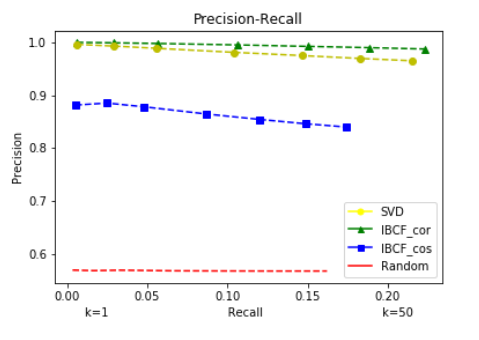
\includegraphics[scale=0.5]{precision_recall.png}}
\caption{Precision Recall of all the models}
\label{fig}
\end{figure}

\section{Conclusion and Discussion}
We have discussed many popular recommendation algorithms \textit{Popularity}, \textit{Collaborative filtering (CF)}, \textit{Content-based filtering (CB)} and, \texit{Hybrid filtering}. Our ambition was to understand pros and cons of each recommendation system algorithms.
It uses different mathematical approaches such as \textit{Pearson co-relation} and \textit{Matrix Factorization} to predict ratings. The problem in predicting ratings while using these algorithms arises due to the sparsity of the matrix and complexity of the computation.
In \textit{Collaborative filtering}, we try to use the user-item rating matrix to predict items to users.  
The problem with \textit{Popularity} recommendation algorithm it recommends same items to all users. The Memory-based models are based on the similarity between users or items. 

As we have seen that the IBCF-correlation (\textit{Item-based collaborative filtering using the correlation distance}) gave best results than any other algorithm. We can also see that all recommendation algorithms performed better than random recommendation.

Theoretically, \textit{SVD (Singular Value Decomposition)} should have performed better than the Item-based approach, because the Low-dimensional recommenders are trying to capture the taste and preferences of the users. However, the performance of SVM model is sensitive not only to some parameters but also to feature subset. Therefore it is very critical to optimize SVM model for more accurate performance. 

\textit{Hybrid Models} could be  used to overcome the shortcomings of a particular model, and are particularly a better approach than single models.

\section*{Acknowledgement}
We offer our sincerest gratitude to our Data Mining professor \textbf{Dr. P. Viswanath} for the Data Mining Course and his encouragement to do \textit{Comparative Study of Different Algorithms Used in Recommender Systems}.

\begin{thebibliography}{00}
\bibitem{b1} Recommendation systems: Principles, methods and
evaluation, F.O. Isinkaye, Y.O. Folajimi, B.A. Ojok, Received 13 March 2015; revised 8 June 2015; accepted 30 June 2015
\bibitem{b2} Isinkaye, F.O., Y.O. Folajimi, and B.A. Ojokoh (2015). ``Recommendation systems: Principles, methods and evaluation". In: Egyptian Informatics Journal 16.3, pp. 261 –273. ISSN: 1110-8665. DOI: https://doi.org/10.1016/j.eij.2015.06.005. 
\bibitem{b3} \href{https://sifter.org/~simon/journal/20061211.html}{https://sifter.org/~simon/journal/20061211.html}
\bibitem{b4} \href{https://link.springer.com/content/pdf/10.1007\%2F11531371_50.pdf}{Sung-Hwan Min and Ingoo Han, Recommender Systems Using Support Vector Machines} 
\bibitem{b8} Breese, J., Heckerman, D., and Kadie, C. (May, 1998). An experimental comparison of collaborative filtering methods. Technical
Report MSR-TR-98-12, Microsoft Research, Redmond, WA.
\bibitem{b9} Yehuda Koren (August 2009). The BellKor Solution to the Netflix Grand Prize.
\bibitem{b10} Yehuda Koren, Robert Bell and Chris Volinsky. (August 2009). Matrix Factorization  Techniques For Recommender Systems.
\bibitem{b11}Girase, Sheetal, Debajyoti Mukhopadhyay, et al. (2015). “Role of Matrix Factorization Model in Collaborative Filtering Algorithm: A Survey”. In: arXiv preprint arXiv:1503.07475. 
\bibitem{b12}\href{http://files.grouplens.org/papers/www10_sarwar.pdf}{Badrul Sarwar, George Karypis, Joseph Konstan, and John Riedl (May 2001). Item-Based Collaborative Filtering Recommendation Algorithms}
\bibitem{b13}Content-based Recommender Systems: State of the Art and Trends, Pasquale Lops, Marco de Gemmis and Giovanni Semeraro
\bibitem{b14}Recommendation System for Netflix, Leidy Esperanza MOLINA, FERNÁNDEZ
\end{thebibliography}
\end{document}
